\documentclass{article}
\usepackage[hmargin=1.1in,vmargin=1in]{geometry}
\usepackage[english]{babel}
\usepackage[utf8x]{inputenc}
\usepackage{mathpazo}
\usepackage{amsmath}
\usepackage{amssymb} 
\usepackage{graphicx}
\usepackage{adjustbox}
\usepackage{tabularx}
\usepackage[flushleft]{threeparttable}
\usepackage{subfig}
\usepackage{kpfonts}    % for nice fonts
\usepackage{microtype} 
\usepackage{booktabs}   % for nice tables
\usepackage{bm}         % for bold math
\usepackage{listings}   % for inserting code
\usepackage{verbatim}   % useful for program listings
\usepackage[colorlinks=true]{hyperref}   % use for hypertext
%\usepackage[hidelinks]{hyperref}         % make links appear black
\usepackage{natbib}
\usepackage{framed}
\usepackage{setspace}
\usepackage{lettrine}
\usepackage{color, soul}
\usepackage{tcolorbox}
\newcommand{\hlc}[2][yellow]{ {\sethlcolor{#1} \hl{#2}} }
\renewcommand{\baselinestretch}{1.3}

\author{
    Erica Myers \thanks{University of Calgary}
    \and
    Maya Papineau \thanks{Carleton University}
    \and
    Nicholas Rivers \thanks{University of Ottawa}
    \and 
    Kareman Yassin \thanks{University of Ottawa}
}

\title{
    Estimates of long-run energy savings and realization rates from a large household energy efficiency retrofit program
}



\begin{document}

\maketitle

\begin{abstract}
	Goes here.
\end{abstract}

\section{Introduction}

\section{Program description}
Describe the EcoEnergy program that we are evaluating.

\section{Data}
We obtain program data for the EcoEnergy Homes program and EnergyGuide for Homes as well as energy consumption data.

The program data is provided by Natural Resources Canada. The data includes all households in Medicine Hat that obtained an energy efficiency audit through the EnerGuide for Homes program. The EnerGuide for homes program is designed to provide a detailed assessment of a home's current energy consumption and to model impacts of energy upgrades on potential energy consumption. Homes go through an in-person audit by an energy efficiency auditor, which includes a physical assessment of the home as well as a blower-door test. Our data includes home measurements and modeled energy consumption.

The program data also includes a record of energy efficiency upgrades that were performed by the household in response to the energy efficiency assessment. In addition, the program data includes a prospective assessment of ex ante expectations of energy savings associated with the suite of upgrades that were undertaken by the homeowner.

The energy consumption data was provided by the City of Medicine Hat, and includes monthly billing data for natural gas and electricity for all homes in the municipality from 2007 to 2019.  The energy consumption data was merged with the program participation data based on address matching.

Summary statistics for the data are provided in Table \ref{tab:sumstat}. The table shows that the data contain observations of 1525 households that participated in the retrofit program, along with 20204 houses that did not participate.  Participant households undertook a number of energy efficiency retrofits, the most popular of which were air sealing, natural gas furnace upgrades, and attic insulation upgrades.  Gas, electricity, and total energy consumption are presented in this table as an annual average over the 13 year period we have data, and include both pre- and post-retrofit observations. The table shows that over this period, there is little difference in energy consumption between participating and non-participating households. As described, the EnerGuide for houses program undertakes detailed engineering calculations to estimate energy consumption both before and following retrofits. Table \ref{tab:sumstat} shows that both pre- and post-retrofit projections of energy consumption are higher than actual energy consumption, indicating a potential bias in the engineering models used to predict energy consumption. Comparing pre- and post-retrofit predictions of energy consumption, we can see that the typical participating household was projected to reduce natural gas consumption by about 28\% and reduce electricity consumption by about 1.3\%. Our analysis is focused on using post-retrofit billing data to determine whether these savings materialized.

\begin{table}[!htbp] \centering \renewcommand*{\arraystretch}{1.1}\caption{Summary statistics\label{tab:sumstat}}\resizebox{\textwidth}{!}{
\begin{tabular}{lrrrrrr}
\hline
\hline
non\_participant & \multicolumn{3}{c}{No} & \multicolumn{3}{c}{Yes}  \\ 
 Variable & \multicolumn{1}{c}{N} & \multicolumn{1}{c}{Mean} & \multicolumn{1}{c}{SD} & \multicolumn{1}{c}{N} & \multicolumn{1}{c}{Mean} & \multicolumn{1}{c}{SD} \\ 
\hline
Energy consumption data & 0 &  &  & 0 &  &  \\ 
Actual gas consumption (GJ/year) & 1453 & 113 & 38 & 18284 & 116 & 41 \\ 
Actual electricity consumption (GJ/year) & 1453 & 31 & 12 & 18284 & 31 & 13 \\ 
Actual energy consumption (GJ/year) & 1453 & 144 & 45 & 18284 & 148 & 48 \\ 
Property assessment data & 0 &  &  & 0 &  &  \\ 
Total assessed value (\$) & 1453 & 276665 & 87090 & 18284 & 289405 & 123025 \\ 
Lot size (square metres) & 1453 & 642 & 294 & 18284 & 816 & 1875 \\ 
Building size (square metres) & 1453 & 118 & 39 & 18284 & 121 & 43 \\ 
Year built & 1453 & 1971 & 18 & 18284 & 1981 & 23 \\ 
Program participation data & 0 &  &  & 0 &  &  \\ 
Air sealing & 1453 & 0.82 & 0.38 & 18284 & 0 & 0 \\ 
Attic insulation & 1453 & 0.64 & 0.48 & 18284 & 0 & 0 \\ 
Wall insulation & 1453 & 0.044 & 0.21 & 18284 & 0 & 0 \\ 
Basement insulation & 1453 & 0.13 & 0.33 & 18284 & 0 & 0 \\ 
Foundation header insulation & 1453 & 0.087 & 0.28 & 18284 & 0 & 0 \\ 
Window or door upgrade & 1453 & 0.18 & 0.39 & 18284 & 0 & 0 \\ 
Central A/C upgrade & 1453 & 0.13 & 0.34 & 18284 & 0 & 0 \\ 
Natural gas furnace upgrade & 1453 & 0.68 & 0.47 & 18284 & 0 & 0 \\ 
Predicted pre-retrofit gas consumption (GJ/year) & 1453 & 161 & 60 & 0 &  &  \\ 
Predicted pre-retrofit electricity consumption (GJ/year) & 1453 & 34 & 1 & 0 &  &  \\ 
Predicted pre-retrofit energy consumption (GJ/year) & 1453 & 195 & 60 & 0 &  &  \\ 
Predicted post-retrofit gas consumption (GJ/year) & 1453 & 116 & 40 & 0 &  &  \\ 
Predicted post-retrofit electricity consumption (GJ/year) & 1453 & 33 & 1.1 & 0 &  &  \\ 
Predicted post-retrofit energy consumption (GJ/year) & 1453 & 149 & 40 & 0 &  & \\ 
\hline
\hline
\end{tabular}
}
\end{table}






\section{Empirical approach}

\subsection{Panel fixed effects analysis}
To estimate the overall impact of participation in the energy efficiency retrofit program, we use a panel fixed effects approach and regress the natural logarithm of monthly energy consumption ($log(e_{iym})$) on an indicator ($\text{retrofit}_{iym}$) that takes on a value of 1 if a household has completed an energy efficiency retrofit under the EnerGuide for Houses program, and zero otherwise. Our main specification includes household fixed effects as well as month-of-sample fixed effects (e.g., February-2017), and takes the following form:
\begin{align}
	log(e_{iym}) = \beta \text{retrofit}_{iym} + \alpha_i + \gamma_{ym} + \epsilon_{iym},
\end{align}
where $i$ indexes households $y$ indexes year, and $m$ indexes month. In all cases, we cluster standard errors on both household as well as month-of-sample.

In this approach, household fixed effects control for time-invariant characteristics of homes in the data set, such as size or orientation, as well as fixed occupant characteristics, such as family size, political orientation, or environmental attitudes. Year-month fixed effects control for time-variant conditions that affect all households equivalently, such as weather (all households are located in the same city, so experience similar weather) or energy prices. The approach is similar to \cite{chuang2022residential}, who evaluate electricity efficiency rebate programs in California, or to \cite{liang2018energy}, who evaluate electricity efficiency programs in Phoenix.\footnote{\cite{chuang2022residential} include house-by-month fixed effects. Using house by month fixed effects does not affect our estimates, as shown in Appendix Table \ref{tab:hm}.}

The coefficient $\hat{\beta}$ that is estimated in the regression analysis is an estimate of the effect of retrofit program participation on energy consumption. The coefficient will identify the true effect of program participation on energy consumption when the so-called ``parallel trends'' assumption holds; that is, when the non-participant households provide a good counterfactual for energy consumption of the participating households had they not undergone the energy efficiency retrofit, conditional on fixed effects. The key potential violation of this assumption occurs because, as in \cite{liang2018energy} and \cite{chuang2022residential} and other similar studies, households self-select into program participation. While we control for time-invariant characteristics that are correlated with participation, such as environmental attitudes, using household fixed effects, there may be house-specific time-varying covariates that determine retrofit program participation, which we cannot observe. For example, households with an old furnace may be more likely to participate in the program, since the value of program participation is likely higher for these households \citep{rivers2016free}. However, these households would have been more likely to replace their furnace anyway, given that it is old. In this case, the estimated $\hat{\beta}$ from the regression will be biased towards larger energy savings than actually occurred \citep{boomhower2014credible}.

\hlc{Think about other potential issues related to identification. Is this infra-marginal issue explained well enough here?}

\subsection{Matched sample analysis}


\subsection{Accounting for staggered adoption}
 

\section{Results}


\subsection{Graphical analysis}
Figure \ref{fig_agg} illustrates long run trends in electricity and natural gas consumption for treated and non-treated households from before and after participation in the energy-efficiency retrofit program. The bottom panel shows that the years 2007 and 2008 were prior to program initiation. The retrofit program began in 2009, and rolled out over the following three years, with all participating households completing retrofits by 2012. Prior to the beginning of the retrofit program (in 2007-08), electricity and gas exhibited similar (annual) trends. Households that would later participate in the retrofit program has higher natural gas consumption and slightly higher electricity consumption than non-participating households. The figure suggests that electricity consumption declined slightly as a result of the retrofits, and that natural gas consumption in treated households fell considerably relative to control households. While the households that chose to participate in retrofits were initially consuming about 5\% more natural gas than non-participant households, after the retrofits they consumed about 3-4\% less natural gas than non-participating households. The change occurred during the retrofit program roll-out (shown in the lower panel of Figure \ref{fig_agg}) and appears to be stable following completion of the roll-out.

\begin{figure}
	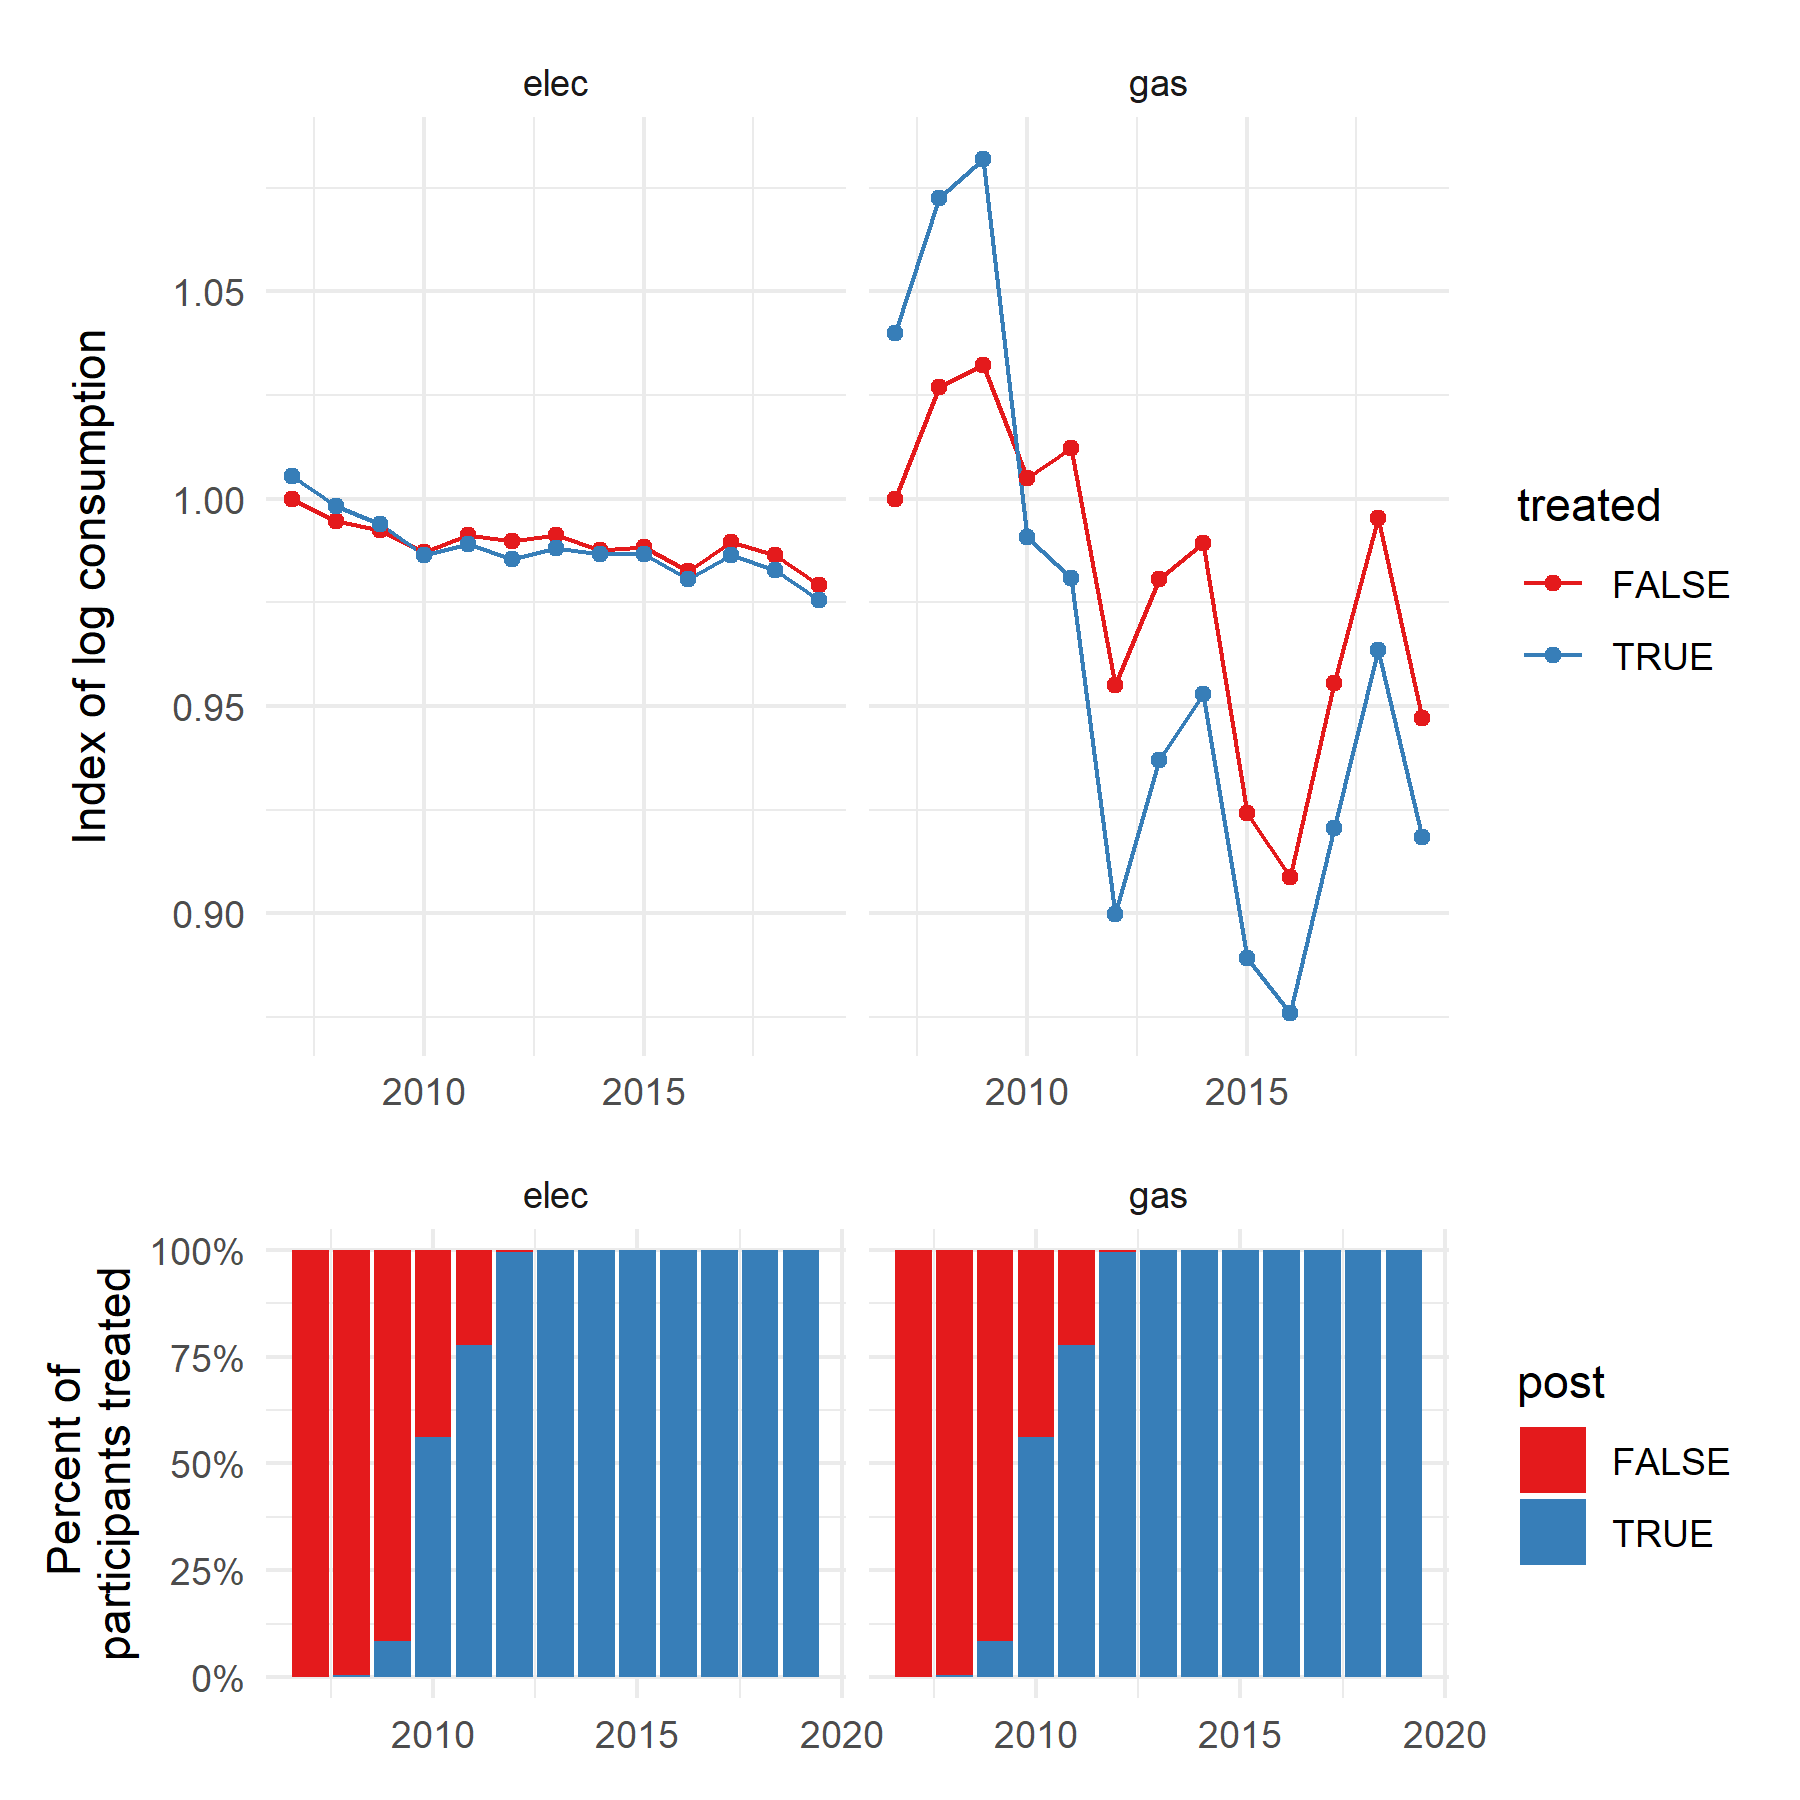
\includegraphics{../output_figures_tables/aggregate_trend_graph}
	\caption{Long-run trends in electricity and natural gas consumption in treated and untreated households}\label{fig_agg}
\end{figure}

{\color{red} Not clear to me why the aggregate trends graph suggests a gas savings of about 10\%, but we are estimating more like 15\%.}


\subsection{Staggered adoption and event studies}
One potential reason for the difference in results with the ever-treated and never-treated samples is because adoption of the energy efficiency measures is staggered over time. Because of the small control group in the ever-treated sample (only a few households retrofit in 2012, and these form the control group in that sample), a large weight is placed on comparisons between newly-treated and previously-treated households. Many papers suggest that these comparisons are potentially problematic, and can result in bias.  We thus conduct our estimation with alternative estimators from Callaway and Sant'a Anna and from Sun and Abraham.  We show results in the form of an event study plot, Figure \ref{fig_esplot}.

The results suggest that the TWFE estimates including the never treated households match well with the Callaway and Sant'a Anna and Sun and Abraham results.  In contrast, the ever-treated sub-sample appears to result in significantly biased coefficients.

\begin{figure}
	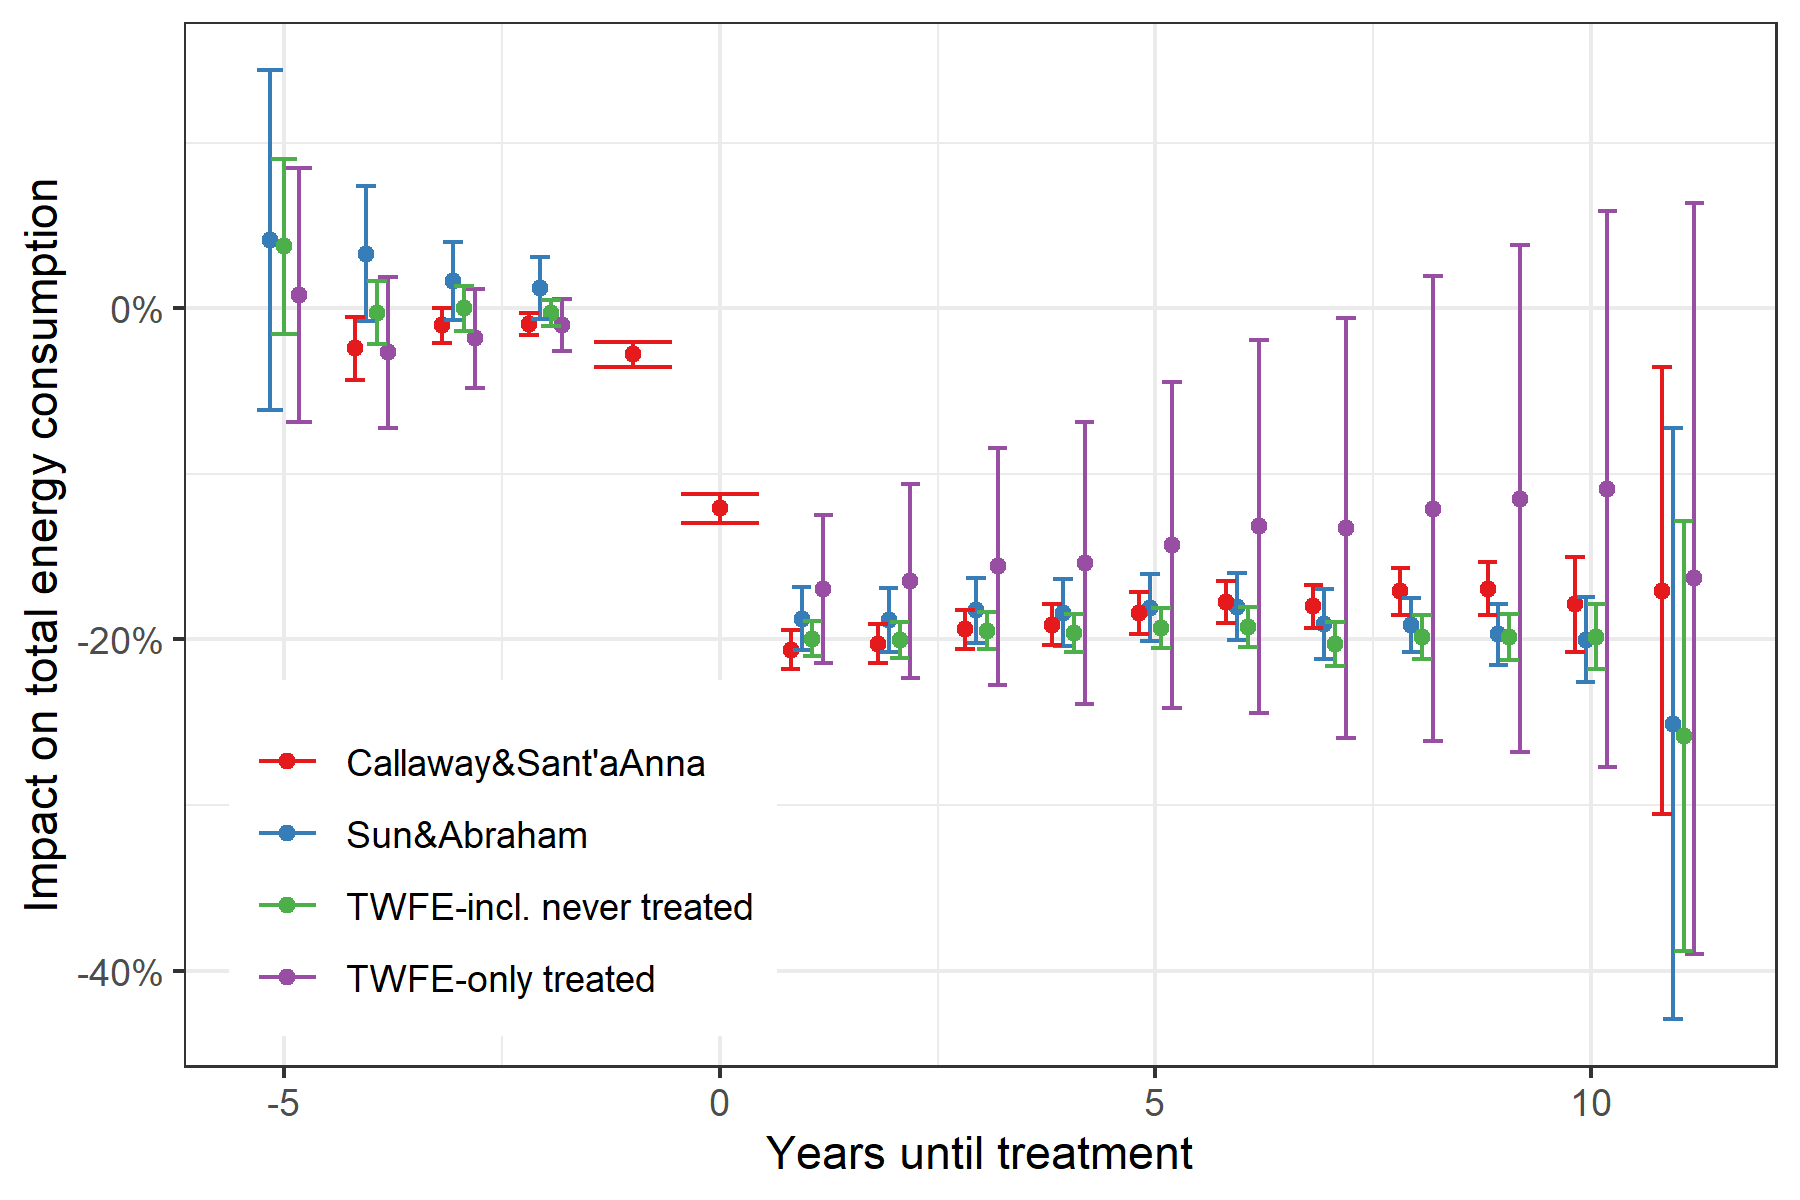
\includegraphics{../output_figures_tables/event_study_plot}
	\caption{Event study plot with different estimation samples and methods}\label{fig_esplot}
\end{figure}


\subsection{Measure specific results}

\subsubsection{Which energy efficiency measures are adopted?}
To estimate projected savings associated with different energy efficiency retrofits, we regress projected energy savings on a vector of dummy variables that indicate whether a measure was implemented:
\begin{align}
	\log y^1_i - \log y^0_i = \sum_j \beta_j x_{ij}.
\end{align}
In the equation, $y^1_i$ is the projected energy consumption of house $i$ after a retrofit is undertaken and $y^0_i$ is projected energy consumption before the retrofit is undertaken. $x_{ij}$ is a dummy variable indicating whether house $i$ implemented retrofit $j$.

Before presenting the results, Figure \ref{fig_corplot} shows a correlation plot of energy efficiency measures. If adoption of measures is highly correlated, it may be difficult to precisely estimate energy savings.  Figure \ref{fig_corplot} shows that for the most part, there is limited correlation between measures.  Only basement insulation and foundation headers are highly correlated.  It may make sense to aggregate these two measures (I haven't done this).

\begin{figure}
	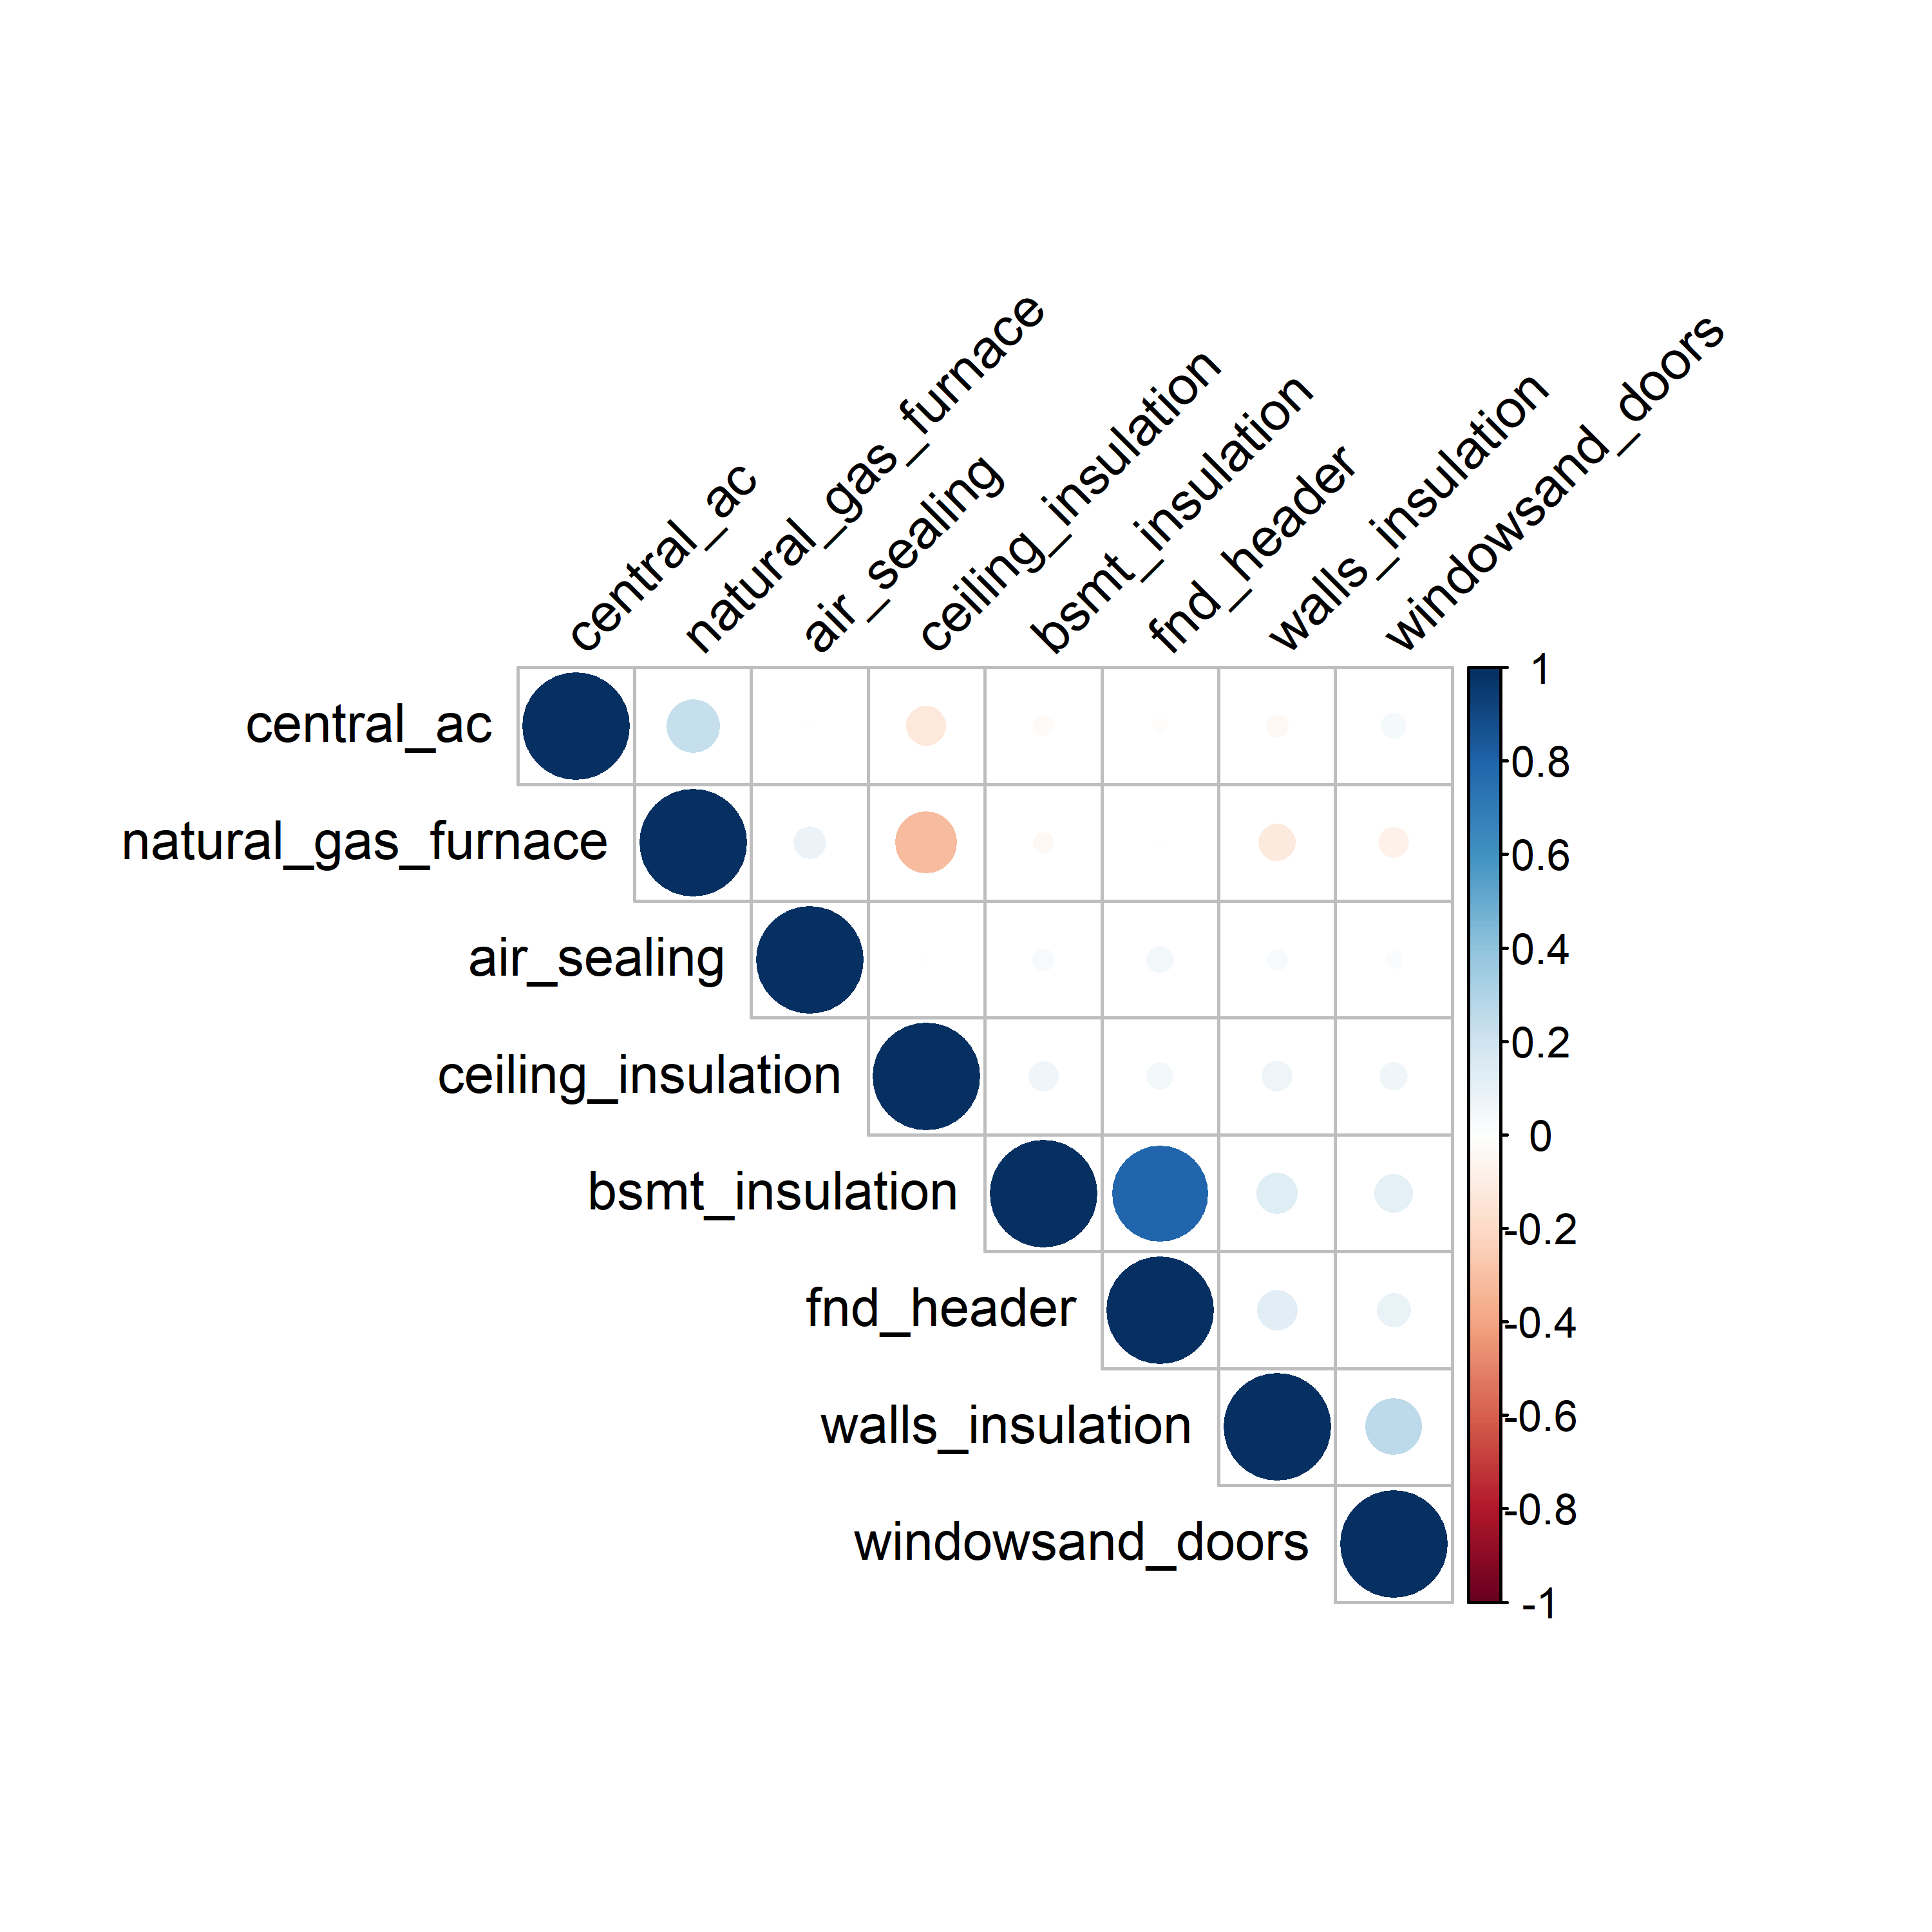
\includegraphics{"../output_figures_tables/correlation_plot.png"}
	\caption{Correlation plot of retrofit measures}\label{fig_corplot}
\end{figure}

Figure \ref{fig_mbm_proj} shows projections of energy savings by measure. Large savings are projected for natural gas furnace upgrades as well as wall insulation.

\begin{figure}
	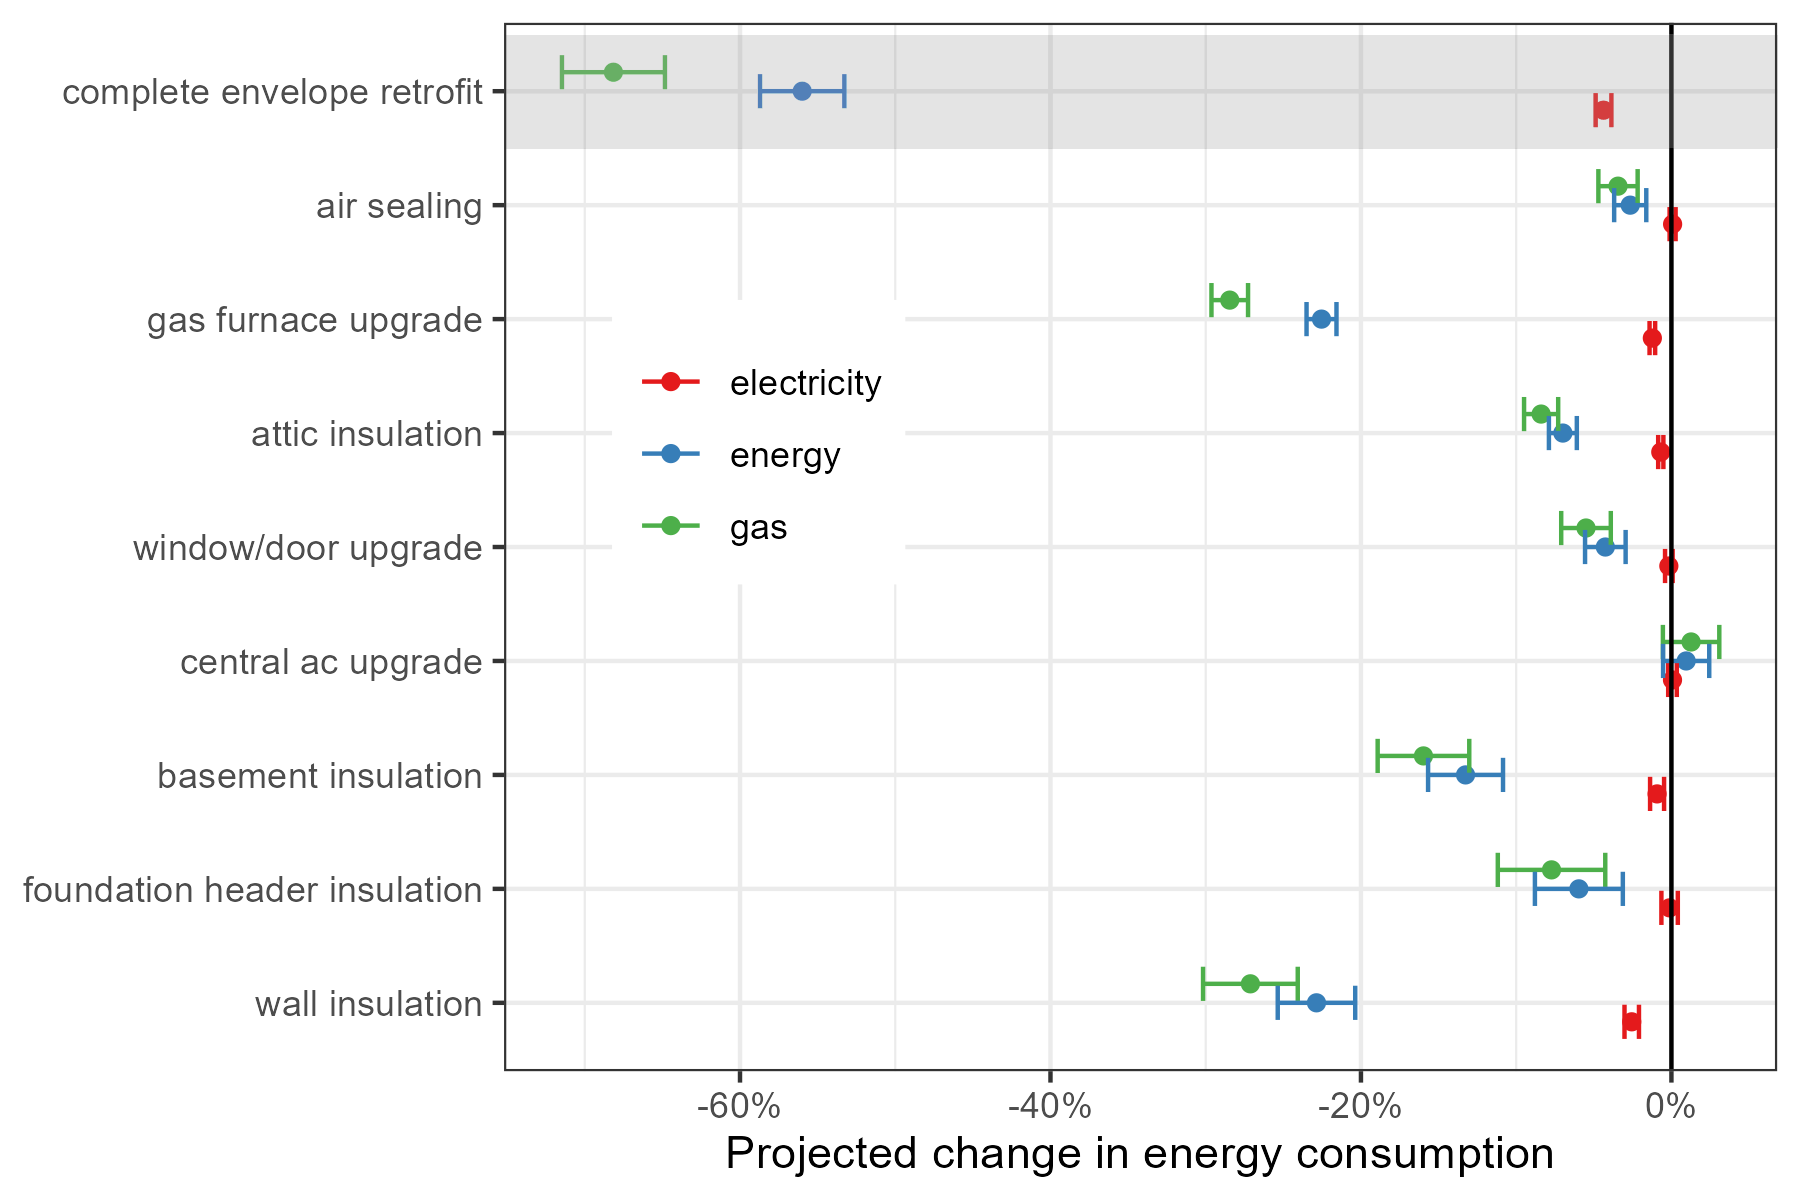
\includegraphics{../output_figures_tables/projected_es_mbm.png}
	\caption{Measure-specific energy saving projections}\label{fig_mbm_proj}
\end{figure}


\subsubsection{Estimated savings}

Figure \ref{fig_proj} shows estimated energy savings from different adopted measures (left panel) and the number of measures adopted (right panel). The largest estimated changes in gas consumption are largest for natural gas furnace upgrades and wall insulation. Air sealing and attic (ceiling) insulation also deliver gas savings that are precisely estimated. In contrast, no measure is shown to save electricity, and walls insulation may actually increase electricity consumption (although few houses adopt walls insulation).

\begin{figure}
	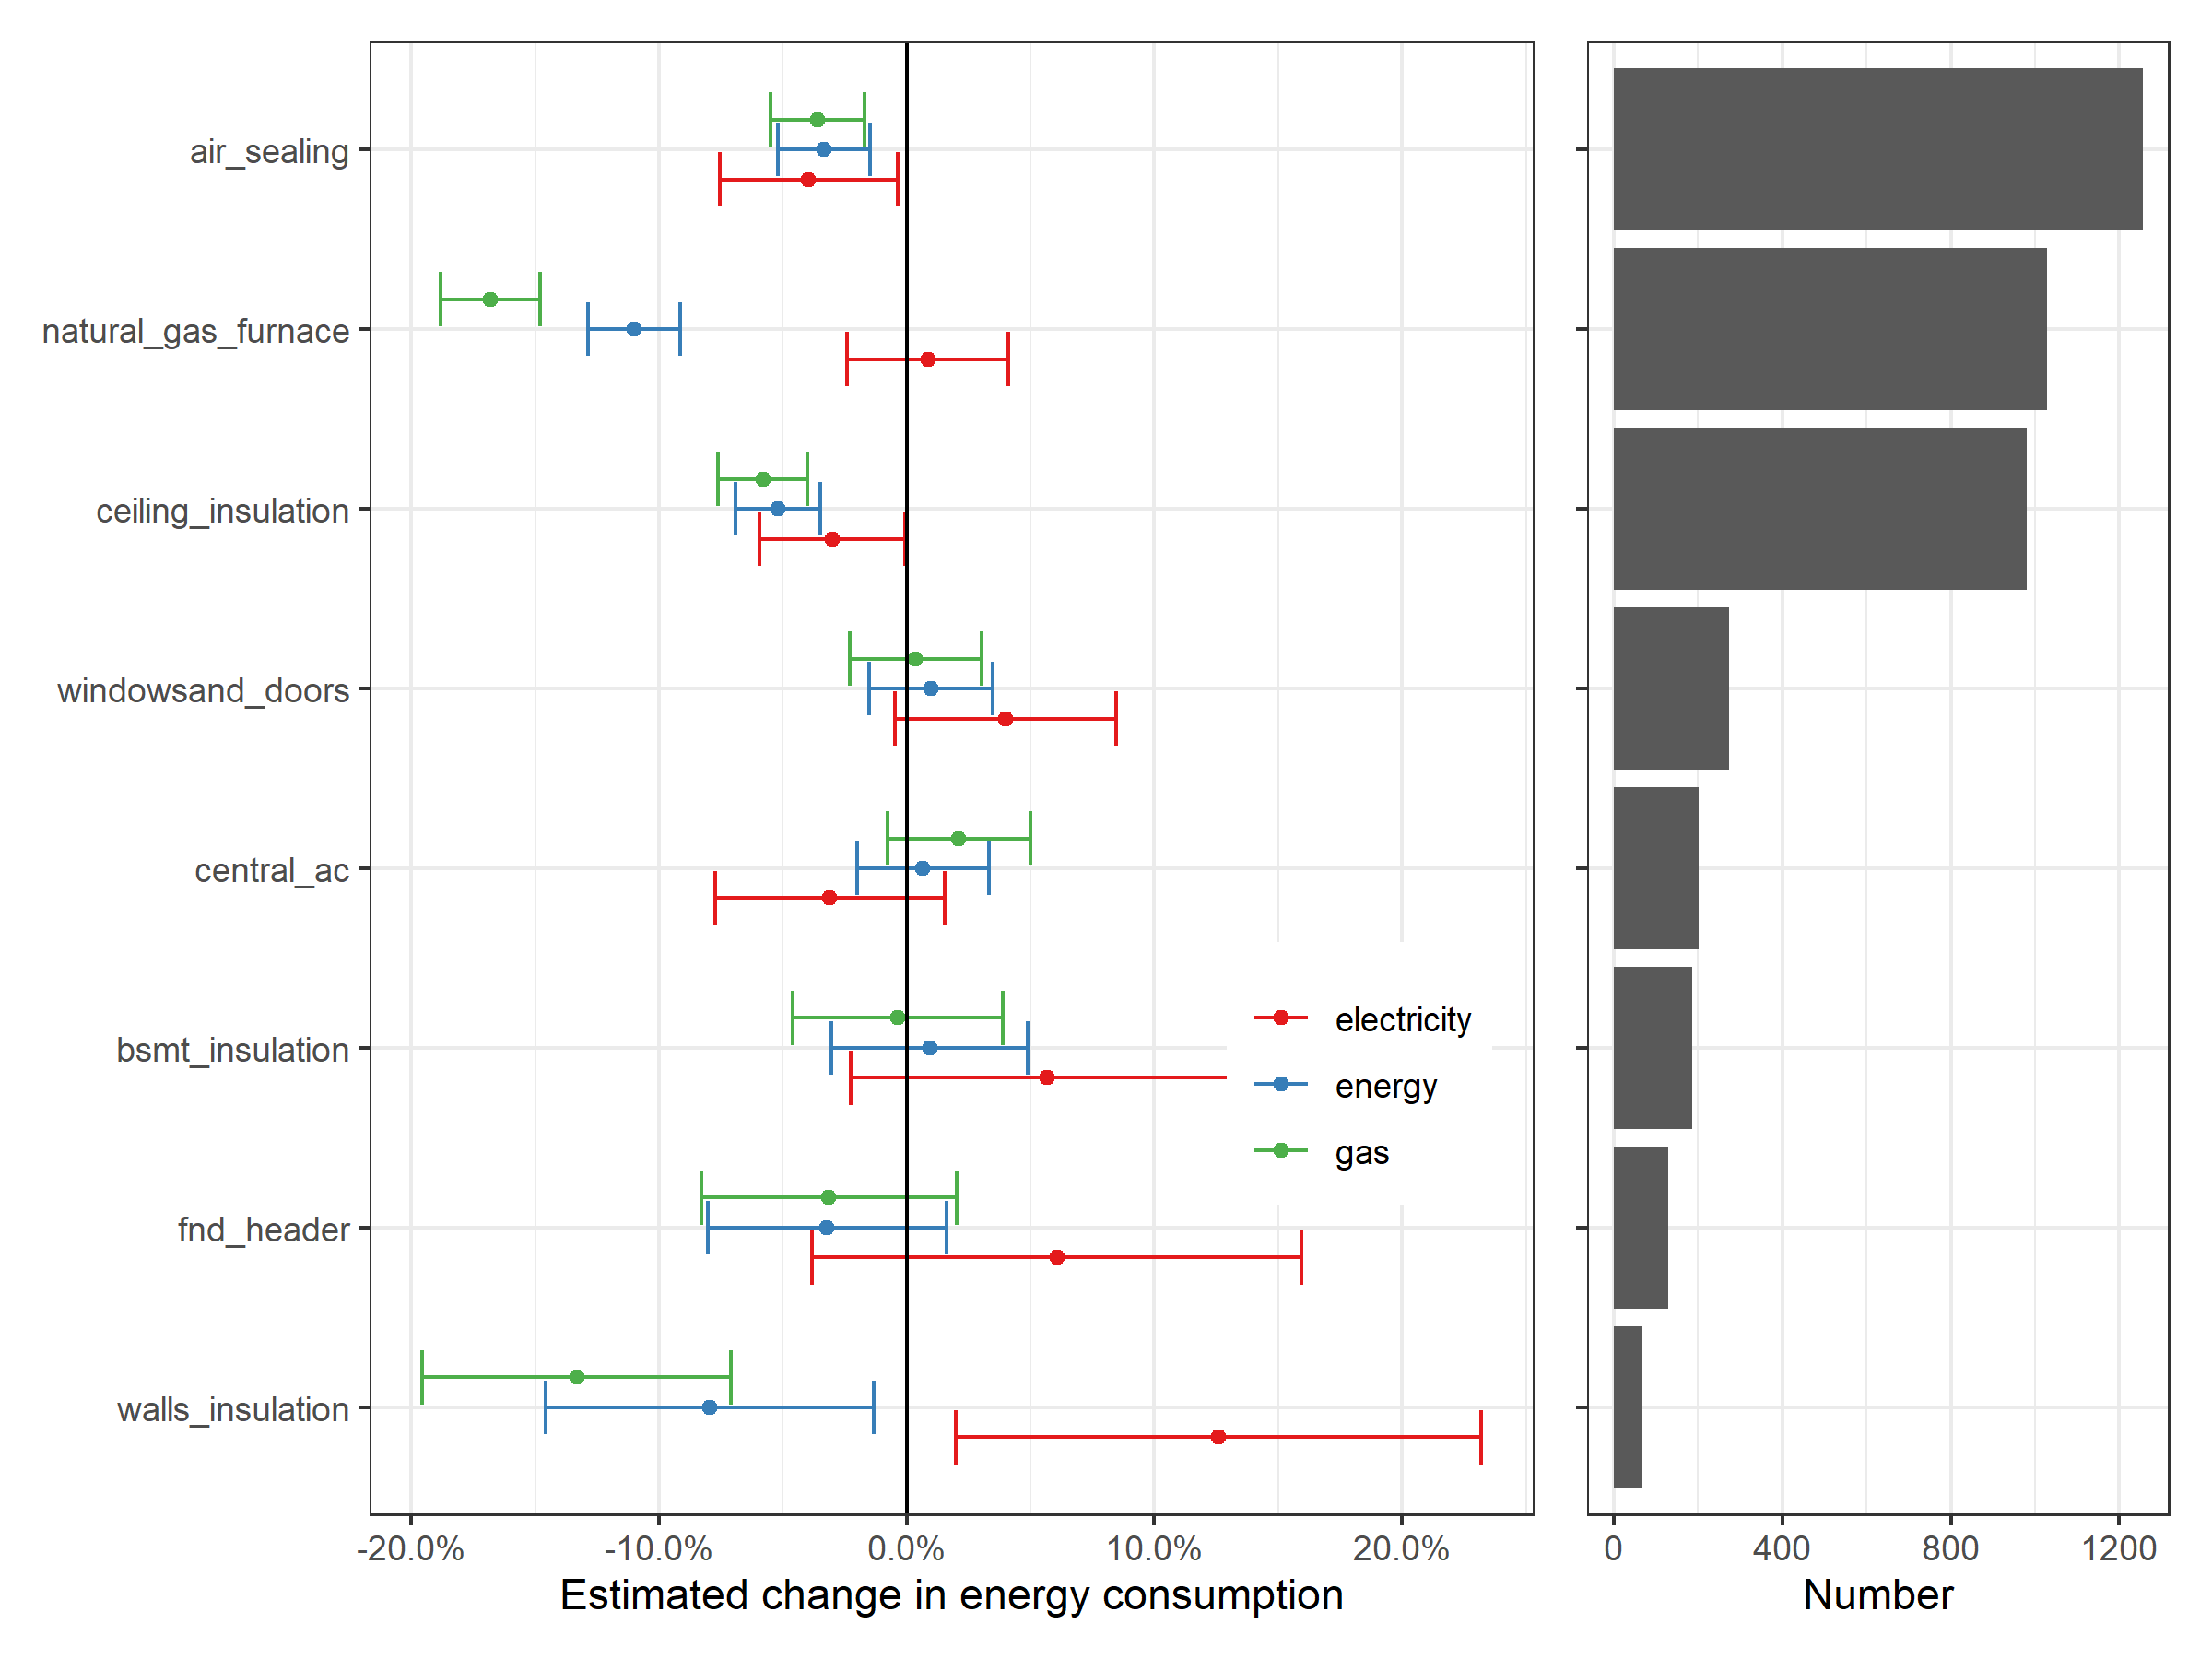
\includegraphics[width=\linewidth]{../output_figures_tables/mbm_energy_savings_combined.png}
	\caption{Estimated energy savings}\label{fig_proj}
\end{figure}


\subsubsection{Realization rates}
We estimate an aggregate realization rate by regressing energy consumption on a post $\times$ treatment dummy interacted with projected energy savings. As shown in the table below, we find a realization rate for natural gas of 50\%. Our realization rate for electricity is negative (we find an increase in electricity consumption, rather than a saving). For all energy, we find a realization rate of 47\%.


\begin{tabular}{lccc}
   \tabularnewline\midrule\midrule
   Dependent Variables:                                & log(gas)       & log(elec)             & log(energy)\\
   Model:                                              & (1)            & (2)                   & (3)\\
   \midrule \emph{Variables} &   &   &  \\
   as.numeric(treated\_post) $\times$ delta\_gas    & 0.6055$^{***}$ &                       &   \\
                                                       & (0.0195)       &                       &   \\
   as.numeric(treated\_post) $\times$ delta\_elec   &                & 0.1226                &   \\
                                                       &                & (0.5118)              &   \\
   as.numeric(treated\_post) $\times$ delta\_energy &                &                       & 0.5464$^{***}$\\
                                                       &                &                       & (0.0276)\\
   \midrule \emph{Fixed-effects} &   &   &  \\
   id                                                  & Yes            & Yes                   & Yes\\
   cons\_date                                         & Yes            & Yes                   & Yes\\
   \midrule \emph{Fit statistics} &   &   &  \\
   Observations                                        & 3,165,406      & 3,208,330             & 3,176,199\\
   R$^2$                                               & 0.84913        & 0.47322               & 0.78446\\
   Within R$^2$                                        & 0.00417        & $4.62\times 10^{-7}$ & 0.00258\\
   \midrule\midrule\multicolumn{4}{l}{\emph{Clustered (id \& cons\_date) standard-errors in parentheses}}\\
   \multicolumn{4}{l}{\emph{Signif. Codes: ***: 0.01, **: 0.05, *: 0.1}}\\
\end{tabular}




We also conduct our analysis in levels rather than logs. Results are shown in the table below, an are similar to the main results in logs.


\begin{tabular}{lccc}
   \tabularnewline\midrule\midrule
   Dependent Variables:                                      & gas            & elec                  & energy\\
   Model:                                                    & (1)            & (2)                   & (3)\\
   \midrule \emph{Variables} &   &   &  \\
   as.numeric(treated\_post) $\times$ delta\_gas\_lev    & 0.6245$^{***}$ &                       &   \\
                                                             & (0.0661)       &                       &   \\
   as.numeric(treated\_post) $\times$ delta\_elec\_lev   &                & 0.0499                &   \\
                                                             &                & (0.4932)              &   \\
   as.numeric(treated\_post) $\times$ delta\_energy\_lev &                &                       & 0.4970$^{***}$\\
                                                             &                &                       & (0.0553)\\
   \midrule \emph{Fixed-effects} &   &   &  \\
   id                                                        & Yes            & Yes                   & Yes\\
   cons\_date                                               & Yes            & Yes                   & Yes\\
   \midrule \emph{Fit statistics} &   &   &  \\
   Observations                                              & 3,192,857      & 3,210,277             & 3,176,946\\
   R$^2$                                                     & 0.75198        & 0.54135               & 0.74822\\
   Within R$^2$                                              & 0.00360        & $1.43\times 10^{-7}$ & 0.00327\\
   \midrule\midrule\multicolumn{4}{l}{\emph{Clustered (id \& cons\_date) standard-errors in parentheses}}\\
   \multicolumn{4}{l}{\emph{Signif. Codes: ***: 0.01, **: 0.05, *: 0.1}}\\
\end{tabular}




Finally, we estimate measure specific realization rates by dividing realized by projected energy savings by measure.  Results are presented in Figure \ref{fig_rr_mbm}. We indicate measure-specific realization rates in percentage form above each measure. For natural gas, we find realizatoin rates of 59\% for furnace upgrades and 51\% for walls insulation. We find a realization rate of above 100\% for air sealing measures. For electricity, we find realization rates that are mostly negative, since most measures appear to be associated with an increase in electricity consumption.

\begin{figure}
	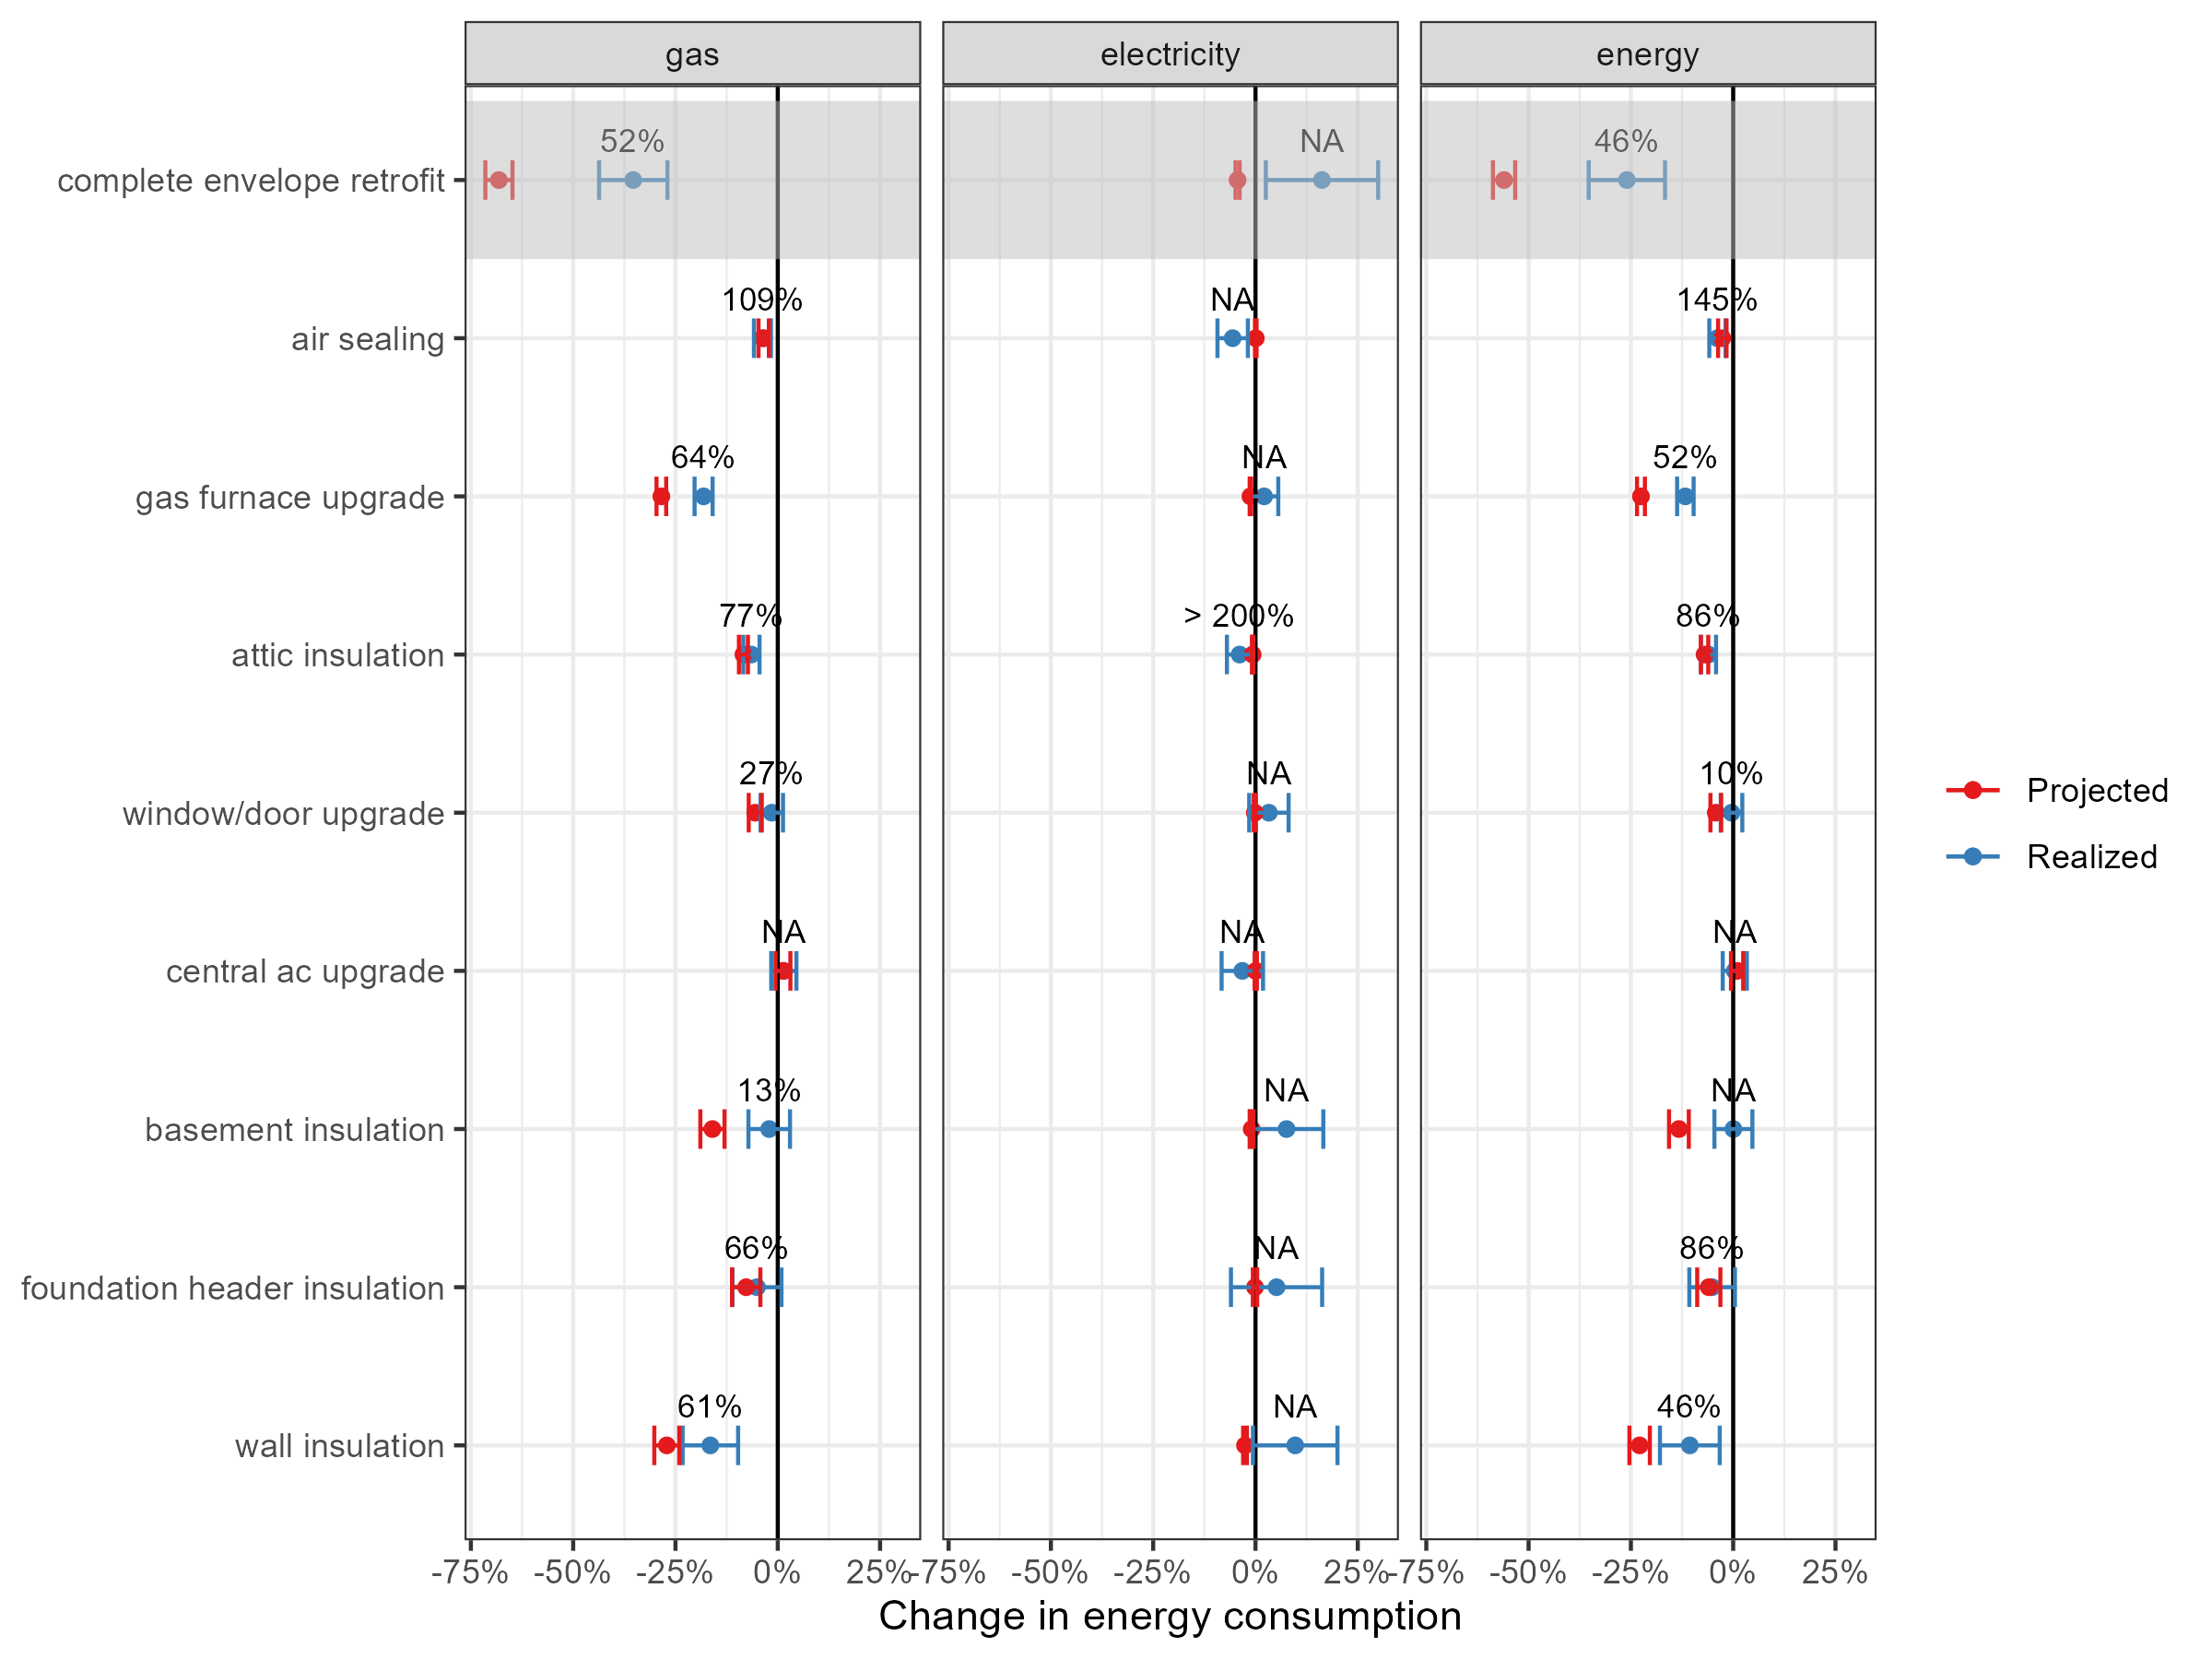
\includegraphics[width=\linewidth]{../output_figures_tables/mbm_realization_rate.png}
	\caption{Measure specific realization rates}\label{fig_rr_mbm}
\end{figure}

\section{Conclusion}

\clearpage
\bibliographystyle{aer}
\bibliography{mh_rr}
\clearpage

\appendix
\section{Additional results}
% Number tables with appendix name
\setcounter{table}{0}
\renewcommand{\thetable}{\Alph{section}\arabic{table}}


\begin{table}[htbp]
   \centering
   \caption{Regression with house-month fixed effects\label{tab:hm}}
   \begin{tabular}{lcc}
      \tabularnewline\midrule\midrule
      Dependent Variable: & \multicolumn{2}{c}{log(energy)}\\
      Model:             & (1)             & (2)\\
      \midrule \emph{Variables} &   &  \\
      treated\_postTRUE & -0.1577$^{***}$ & -0.1579$^{***}$\\
                         & (0.0063)        & (0.0063)\\
      \midrule \emph{Fixed-effects} &   &  \\
      id                 & Yes             & \\
      cons\_date        & Yes             & Yes\\
      id-consmonth       &                 & Yes\\
      \midrule \emph{Fit statistics} &   &  \\
      Observations       & 2,926,828       & 2,926,828\\
      R$^2$              & 0.79168         & 0.84947\\
      Within R$^2$       & 0.00269         & 0.00371\\
      \midrule\midrule\multicolumn{3}{l}{\emph{Clustered (id \& cons\_date) standard-errors in parentheses}}\\
      \multicolumn{3}{l}{\emph{Signif. Codes: ***: 0.01, **: 0.05, *: 0.1}}\\
   \end{tabular}
\end{table}




\end{document}